%----------------------------------------
%
%  Calendar
%
%  R. Layton
%  2013-12-14
%  rev. 2017-08-25
%
%----------------------------------------PREAMBLE
\documentclass[oneside]{tufte-handout}\usepackage[]{graphicx}\usepackage[]{color}
%% maxwidth is the original width if it is less than linewidth
%% otherwise use linewidth (to make sure the graphics do not exceed the margin)
\makeatletter
\def\maxwidth{ %
  \ifdim\Gin@nat@width>\linewidth
    \linewidth
  \else
    \Gin@nat@width
  \fi
}
\makeatother

\definecolor{fgcolor}{rgb}{0.345, 0.345, 0.345}
\newcommand{\hlnum}[1]{\textcolor[rgb]{0.686,0.059,0.569}{#1}}%
\newcommand{\hlstr}[1]{\textcolor[rgb]{0.192,0.494,0.8}{#1}}%
\newcommand{\hlcom}[1]{\textcolor[rgb]{0.678,0.584,0.686}{\textit{#1}}}%
\newcommand{\hlopt}[1]{\textcolor[rgb]{0,0,0}{#1}}%
\newcommand{\hlstd}[1]{\textcolor[rgb]{0.345,0.345,0.345}{#1}}%
\newcommand{\hlkwa}[1]{\textcolor[rgb]{0.161,0.373,0.58}{\textbf{#1}}}%
\newcommand{\hlkwb}[1]{\textcolor[rgb]{0.69,0.353,0.396}{#1}}%
\newcommand{\hlkwc}[1]{\textcolor[rgb]{0.333,0.667,0.333}{#1}}%
\newcommand{\hlkwd}[1]{\textcolor[rgb]{0.737,0.353,0.396}{\textbf{#1}}}%
\let\hlipl\hlkwb

\usepackage{framed}
\makeatletter
\newenvironment{kframe}{%
 \def\at@end@of@kframe{}%
 \ifinner\ifhmode%
  \def\at@end@of@kframe{\end{minipage}}%
  \begin{minipage}{\columnwidth}%
 \fi\fi%
 \def\FrameCommand##1{\hskip\@totalleftmargin \hskip-\fboxsep
 \colorbox{shadecolor}{##1}\hskip-\fboxsep
     % There is no \\@totalrightmargin, so:
     \hskip-\linewidth \hskip-\@totalleftmargin \hskip\columnwidth}%
 \MakeFramed {\advance\hsize-\width
   \@totalleftmargin\z@ \linewidth\hsize
   \@setminipage}}%
 {\par\unskip\endMakeFramed%
 \at@end@of@kframe}
\makeatother

\definecolor{shadecolor}{rgb}{.97, .97, .97}
\definecolor{messagecolor}{rgb}{0, 0, 0}
\definecolor{warningcolor}{rgb}{1, 0, 1}
\definecolor{errorcolor}{rgb}{1, 0, 0}
\newenvironment{knitrout}{}{} % an empty environment to be redefined in TeX

\usepackage{alltt}

\title{Calendar}
\author{  }
\date{  }

%----------------------------------------INITIALIZE




% Input LaTeX packages
% the .Rnw file location is the working directory for LaTeX commands
% LaTeX packages

%\hypersetup{colorlinks}	 % colored hyperlinks for onscreen viewing
\usepackage{booktabs} 	
\usepackage{ctable}       % for use with xtable printing
\usepackage{pdfpages}

\usepackage{sistyle}
\SIthousandsep{,}

% plus all the packages invoked by the Tufte handout class



% new commands
\newcommand{\NL}{\newthought{}}

% add the course logo
\newcommand{\DataVizLogo}{%
\marginnote[-4\baselineskip]{\raggedleft\small
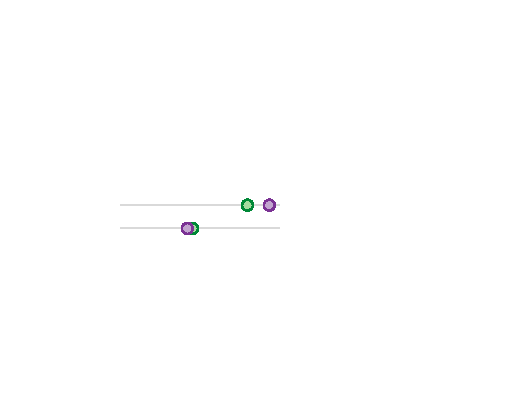
\includegraphics[scale=1.1]{../common/CourseLogo3a.pdf}\\
{\em \Large Visualizing Data} \\ 
\thisterm \\ 
R. Layton\\
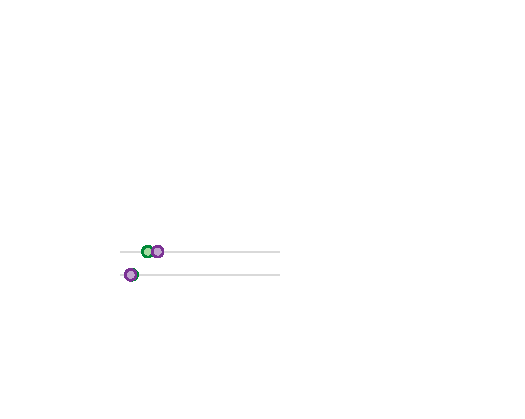
\includegraphics[scale=1.1]{../common/CourseLogo3b.pdf}
}%
}%

\usepackage{bbding} % for dingbats




%----------------------------------------DESCRIPTION
\IfFileExists{upquote.sty}{\usepackage{upquote}}{}
\begin{document}
\begin{fullwidth}

% latex table generated in R 3.4.1 by xtable 1.8-2 package
% Mon Aug 28 16:06:36 2017
\begin{table}[ht]
\centering
\begingroup\small
\begin{tabular}{>{\centering}m{3.5mm}>{\centering\sc}m{2.5mm}m{47mm}m{65mm}m{33mm}@{}}
  \toprule Wk &   & Agenda & Reading \& activities for steady progress & Complete before class \\ 
  \midrule 0 & r & Course goals \& outcomes & Handout the Tufte booklets &  \\ 
    & f & Introduction to visual rhetoric & Syllabus, calendar, and about the portfolio & [tut] R/Rstudio access \\ 
   \midrule 1 & m & [tut] D1 Scatterplots & Ch 2: Limitations of common graphs & [tut] Starting with R \\ 
    & t & [tut] Data basics &  &  \\ 
    & r & Discuss today's reading: & Tufte (1997) Challenger launch decision & Written response form \\ 
    & f & [tut] Markdown basics & Browse the sample portfolio entries &  \\ 
   \midrule 2 & m & [tut] D2 Dot plots & Wk 1 tutorials done. D1+critique in-progress. &  \\ 
    & t & [tut] Subsetting data & Ch 4: Some more effective graphs &  \\ 
    & r & Present and discuss D1+critique &  & D1 (bring to class) \\ 
    & f & [tut] Document design 1 & Kostelnick (1998) Conflicting standards &  \\ 
   \midrule 3 & m & [tut] D3 Multiways & Wk 2 tutorials done. D2+critique in-progress. &  \\ 
    & t & [tut] Reshaping data &  &  \\ 
    & r & Discuss today's reading: & Kostelnick (2007) The conundrum of clarity & Written response form \\ 
    & f & [tut] Basic file management & Ch 5: More than two variables & D2 (turn in) \\ 
   \midrule 4 & m & [tut] Finding interesting data & Wk 3 tutorials done. D3+critique in-progress. &  \\ 
    & t & [tut] D4 Tables & Few (2012) Differing roles of tables \& graphs &  \\ 
    & r & Present and discuss D3+critique &  & D3 (bring to class) \\ 
    & f & Visual lies & Wainer (1997) How to display data badly &  \\ 
   \midrule 5 & m & [tut] D5 Box plots & Wk 4 tutorials done. D4+critique in-progress. &  \\ 
    & t & [tut] Match display to data type & Doumont (2009) Designing the graph &  \\ 
    & r & Discuss today's reading: & Wainer (2014) 15 displays about one thing & Written response form \\ 
    & f & [tut] Document design 2 &  & D4 (turn in) \\ 
   \midrule 6 & m & [tut] D6 Small multiples & Wk 5 tutorials done. D5+critique in-progress. &  \\ 
    & t & Tufte on design & Ch 6: General design principles &  \\ 
    & r & (Fall break) &  &  \\ 
    & f & (Fall break) & Catch up on tutorials or readings. & D5 (turn in) \\ 
   \midrule 7 & m & [tut] D7/D8 Beyond basic graphs & Wk 6 tutorials done. D6+critique in-progress. &  \\ 
    & t & [tut] Color & Constable (2017) Color &  \\ 
    & r & Present and discuss D6+critique & Begin revising displays and critiques & D6 (bring to class) \\ 
    & f & Work on portfolio & Ch 7: Scales &  \\ 
   \midrule 8 & m & [tut] D7/D8 Original displays & Wk 7 tutorials done. D7+critique in-progress. &  \\ 
    & t & Revising displays and critiques & Continue revising displays and critiques &  \\ 
    & r & Discuss today's reading: & Dragga \& Voss (2001) Cruel pies & Written response form \\ 
    & f & [tut] Front \& back matter & Ch 8: Before and after examples & D7 (turn in) \\ 
   \midrule 9 & m & Current topics in data science & Wk 8 tutorials done. D8+critique in-progress. &  \\ 
    & t & Discovering stories in data & Knaflic (2012) So what? &  \\ 
    & r & Present and discuss D8+critique &  & D8 (bring to class) \\ 
    & f & Work on portfolio & Continue revising displays and critiques &  \\ 
   \midrule 10 & m & Current topics in data science & Ch 10: Graphical choices &  \\ 
    & t & Evals \& work on portfolio & Continue revising displays and critiques &  \\ 
    & r & Discuss today's reading: & Spence (2006) William Playfair & Written response form \\ 
    & f & Work on portfolio & Continue revising displays and critiques &  \\ 
   \midrule 11 & w & Submit final portfolio &  & Portfolio \\ 
   \bottomrule   &  &  & Notes: &  \\ 
    &  &  & A written critique accompanies every display. &  \\ 
    &  &  & [tut] denotes a tutorial. &  \\ 
  \end{tabular}
\endgroup
\end{table}

\FloatBarrier

\end{fullwidth}
\end{document}
